\documentclass[11pt, reqno]{amsart}
\usepackage[english]{babel}

\usepackage{layout}
\usepackage{afterpage}
\usepackage[
  asymmetric,
  textheight     = 673pt,
  marginparsep   = 7pt,
  footskip       = 27pt,
  hoffset        = 0pt,
  paperwidth     = 597pt,
  textwidth      = 452pt,
  marginparwidth = 101pt,
  voffset        = 0pt,
  paperheight    = 845pt,
]{geometry}

% Math stuff: do not mess with the ordering!
\usepackage{tikz}
\usepackage{mathtools}
\usepackage{amsthm}
\usepackage{amssymb}
\usepackage{stmaryrd}
\usepackage{tikz-cd}
\usepackage{tqft}

% Font
\usepackage[no-math]{newpxtext}
\usepackage{newpxmath}
% Set arrow tip to that of newpxmath
\tikzset{>=Straight Barb, commutative diagrams/arrow style=tikz}

% Utilities
\usepackage{enumerate}
\usepackage{todonotes}
\usepackage{graphicx}

% Color
\usepackage{xcolor}
\definecolor{brightmaroon}{rgb}{0.76, 0.13, 0.28}

% References
\usepackage{hyperref}
\hypersetup{
  colorlinks = true,
  allcolors  = brightmaroon,
}
\usepackage[capitalize,nameinlink]{cleveref}
\usepackage[
  backend = biber,
  style   = alphabetic,
]{biblatex}
\addbibresource{bibliography.bib}

% Table of contents: show subsections
\setcounter{tocdepth}{2}

\linespread{1.05}
\vfuzz=14pt % No more vbox errors all over the place

%%%%%%%%%%%%%%%%%%%%%%%%%%%%%%%%%%%%%%%%%%%%%%%%%%%%%%%%%%%%%%%%%%%%%%%%%%%%%%%
% ** Environments **

\theoremstyle{definition}
\newtheorem{theorem}{Theorem}[section]
\newtheorem{proposition}[theorem]{Proposition}
\newtheorem{lemma}[theorem]{Lemma}
\newtheorem{corollary}[theorem]{Corollary}
\newtheorem{axiom}[theorem]{Axiom}
\newtheorem{definition}[theorem]{Definition}
\newtheorem{remark}[theorem]{Remark}
\newtheorem{example}[theorem]{Example}
\newtheorem{notation}[theorem]{Notation}

%%%%%%%%%%%%%%%%%%%%%%%%%%%%%%%%%%%%%%%%%%%%%%%%%%%%%%%%%%%%%%%%%%%%%%%%%%%%%%%
% ** symbols **

\renewcommand{\qedsymbol}{\(\natural\)}
\renewcommand{\leq}{\leqslant}
\renewcommand{\geq}{\geqslant}
\renewcommand{\setminus}{\smallsetminus}
\renewcommand{\preceq}{\preccurlyeq}

% ':' for maps and '\colon' for relations on collections
\DeclareMathSymbol{:}{\mathpunct}{operators}{"3A}
\let\colon\relax
\DeclareMathSymbol{\colon}{\mathrel}{operators}{"3A}

% Disjoint unions over sets
\newcommand{\disj}{\amalg}     % Disjoint union
\newcommand{\bigdisj}{\coprod} % Indexed disjoint union

\DeclareMathOperator{\Log}{Log}
\newcommand{\img}{\text{i}}

% Constant map
\DeclareMathOperator{\const}{cons}

% Multiplication map
\DeclareMathOperator{\mul}{mul}

\DeclareMathOperator{\Bd}{\partial}
\DeclareMathOperator{\Cyl}{Cyl}

%%%%%%%%%%%%%%%%%%%%%%%%%%%%%%%%%%%%%%%%%%%%%%%%%%%%%%%%%%%%%%%%%%%%%%%%%%%%%%%
% ** arrows **

% Alias for Rightarrow
\newcommand{\To}{\Rightarrow}

% Monomorphism arrow
\newcommand{\mono}{\rightarrowtail}

% Epimorphism arrow
\newcommand{\epi}{\twoheadrightarrow}

% Unique morphism
\newcommand{\unique}{\to}%{\dashrightarrow}
\newcommand{\xdashrightarrow}[2][]{\ext@arrow 0359\rightarrowfill@@{#1}{#2}}

% Isomorphism symbol
\newcommand{\iso}{\simeq}

\newcommand{\arrowiso}{\iso}
% Isomorphism arrow
\newcommand{\isoto}{\xrightarrow{\raisebox{-.6ex}[0ex][0ex]{\(\arrowiso\)}}}

% How isomorphisms are depicted in diagrams: either \sim or \simeq
\newcommand{\dis}{\iso}

\newcommand{\isounique}{%
  \xdashrightarrow{\raisebox{-.6ex}[0ex][0ex]{\(\arrowiso\)}}
}%

% Natural transformation arrow
\newcommand{\nat}{\Rightarrow}

% Natural isomorphism
\newcommand{\isonat}{\xRightarrow{\raisebox{-.6ex}[0ex][0ex]{\(\arrowiso\)}}}

% Embedding arrow
\newcommand{\emb}{\hookrightarrow}

% Parallel arrows
\newcommand{\para}{\rightrightarrows}

% Adjoint arrows
\newcommand{\adj}{\rightleftarrows}

% Implication
\renewcommand{\implies}{\Rightarrow}
\renewcommand{\impliedby}{\Leftarrow}

% Limits
\DeclareMathOperator{\Lim}{lim}     % Limit
\DeclareMathOperator{\Colim}{colim} % Colimit
\DeclareMathOperator{\Eq}{eq}       % Equalizer
\DeclareMathOperator{\Coeq}{coeq}   % Coequalizer

%%%%%%%%%%%%%%%%%%%%%%%%%%%%%%%%%%%%%%%%%%%%%%%%%%%%%%%%%%%%%%%%%%%%%%%%%%%%%%%
% ** Common collections **

\newcommand{\Z}{\mathbf{Z}}
\newcommand{\N}{\mathbf{N}}
\newcommand{\Q}{\mathbf{Q}}
\newcommand{\CC}{\mathbf{C}}
\newcommand{\R}{\mathbf{R}}
\newcommand{\FF}{\mathbf{F}}

\renewcommand{\emptyset}{\varnothing}

\newcommand{\Uhs}{\mathbf{H}}  % Upper half space
\newcommand{\Proj}{\mathbf{P}} % Projective space

%%%%%%%%%%%%%%%%%%%%%%%%%%%%%%%%%%%%%%%%%%%%%%%%%%%%%%%%%%%%%%%%%%%%%%%%%%%%%%%
% ** Categories **

% Font for categories
\newcommand{\cat}{\texttt}
\newcommand{\catfont}{\texttt}

% Opposite category
\newcommand{\op}{\mathrm{op}}

% Common categories
\newcommand{\Set}{{\catfont{Set}}}          % Sets
\newcommand{\FinSet}{{\catfont{FinSet}}}    % Finite sets
\newcommand{\pSet}{{\catfont{pSet}}}        % Pointed sets
\newcommand{\tOrd}{{\catfont{tOrd}}}        % Totally ordered sets

\newcommand{\Vect}{{\catfont{Vect}}}        % Vector spaces
\newcommand{\FinVect}{{\catfont{FinVect}}}  % Finite vector spaces

\newcommand{\TVect}{{\catfont{TVect}}}      % Topological vector spaces
\newcommand{\Ban}{{\catfont{Ban}}}          % Banach spaces

\newcommand{\Grp}{{\catfont{Grp}}}          % Groups
\newcommand{\Ab}{{\catfont{Ab}}}            % Abelian groups
\newcommand{\GSet}[1]{{{#1}\text{-}\Set}}   % G-sets
\newcommand{\Grpd}{{\catfont{Grpd}}}        % Groupoids

\newcommand{\Mon}{{\catfont{Mon}}}          % Monoidal category
\newcommand{\coMon}{{\catfont{coMon}}}      % coMonoidal category
\newcommand{\rActMon}{{\catfont{rActMon}}}  % right action category
\newcommand{\lActMon}{{\catfont{lActMon}}}  % left action category
\newcommand{\BrMonCat}{{\catfont{BrMonCat}}} % Cat of braided monoidal cats

\newcommand{\Graph}{{\catfont{Graph}}}      % Graphs
\newcommand{\SimpGraph}{{\catfont{sGraph}}} % Simple graphs
\newcommand{\ProfCol}{{\catfont{Prof}(\Col)}}   % C-profile category


\newcommand{\Rng}{{\catfont{Ring}}}             % Rings
\newcommand{\cRng}{{\catfont{CRing}}}           % Commutative rings
\newcommand{\rMod}[1]{{\texttt{Mod}_{#1}}}      % Right modules
\newcommand{\lMod}[1]{{{}_{#1}\catfont{Mod}}}   % Left modules
\newcommand{\Mod}[1]{{#1\text{-}\catfont{Mod}}} % Modules over comm. ring
\newcommand{\Alg}[1]{{#1\text{-}\catfont{Alg}}} % Algebras
\newcommand{\cAlg}[1]{{#1\text{-}\catfont{CAlg}}} % Commutative algebras

\newcommand{\Psh}[1]{{\catfont{Psh}({#1})}}   % Category of presheaves
\newcommand{\comma}{\downarrow} % Comma category separator
\DeclareMathOperator{\El}{El}              % Category of elements

% Operators
\DeclareMathOperator{\Hom}{Mor}   % Morphisms
\DeclareMathOperator{\Mono}{Mono} % Monomorphisms
\DeclareMathOperator{\Epi}{Epi}   % Epimorphisms
\DeclareMathOperator{\Fct}{Fct}   % Functors
\DeclareMathOperator{\Obj}{Obj}   % Objects
\DeclareMathOperator{\Mor}{Mor}   % Morphisms, again
\DeclareMathOperator{\End}{End}   % Endomorphisms
\DeclareMathOperator{\Aut}{Aut}   % Automorphisms
\DeclareMathOperator{\Id}{id}     % Identity
\DeclareMathOperator{\im}{im}     % Image
\DeclareMathOperator{\dom}{dom}   % Domain
\DeclareMathOperator{\codom}{cod} % Codomain

%%%%%%%%%%%%%%%%%%%%%%%%%%%%%%%%%%%%%%%%%%%%%%%%%%%%%%%%%%%%%%%%%%%%%%%%%%%%%%%
% ** algebra **
\DeclareMathOperator{\rank}{rank}
\DeclareMathOperator{\coker}{coker}
\DeclareMathOperator{\codim}{codim}
\DeclareMathOperator{\Tr}{tr}   % Trace
\DeclareMathOperator{\Sym}{Sym} % Symmetric space
\DeclareMathOperator{\Alt}{Alt} % Alternating space
\DeclareMathOperator{\Ann}{Ann} % Annihilator
\DeclareMathOperator{\Char}{char}
\DeclareMathOperator{\Span}{span}
\DeclareMathOperator{\Inn}{Inn}     % Inner automorphisms

\DeclareMathOperator{\eval}{eval}
\DeclareMathOperator{\sign}{sign}

% Matrices
\DeclareMathOperator{\Mat}{Mat}
\DeclareMathOperator{\GL}{GL}
\DeclareMathOperator{\SL}{SL}
\DeclareMathOperator{\PSL}{PSL}
\DeclareMathOperator{\SO}{SO}
\DeclareMathOperator{\SU}{SU}
\DeclareMathOperator{\Unit}{U}
\DeclareMathOperator{\Orth}{O}

% Symbol for the group of units --- for instance, the group of units of a ring
% \(R\) will be denoted by \(R^{\unit}\).
\newcommand{\unit}{\times}

% Orbit and stabilizer
\DeclareMathOperator{\Orb}{Orb}
\DeclareMathOperator{\Stab}{Stab}

% Left and right group actions
\newcommand{\laction}{\circlearrowright}
\newcommand{\raction}{\circlearrowleft}

% Ring ideals font
\newcommand{\ideal}[1]{\mathfrak{#1}}

%%%%%%%%%%%%%%%%%%%%%%%%%%%%%%%%%%%%%%%%%%%%%%%%%%%%%%%%%%%%%%%%%%%%%%%%%%%%%%%
% ** Topology **

\let\Top\relax
\newcommand{\Top}{{\catfont{Top}}}                       % Topological spaces
\newcommand{\Cob}[1]{{#1}\text{-}{\catfont{cob}}} % Cobordisms
\newcommand{\tqft}[1]{{#1}\text{-}{\catfont{TQFT}}} % Cobordisms
\newcommand{\Frob}{{\catfont{Frob}}} % Frobenius algebras
\newcommand{\cFrob}{{\catfont{cFrob}}} % Commutative Frobenius algebras
\newcommand{\SymMon}{{\catfont{SymMon}}} % Symmetric monoidal functor category

% attaching spaces
\newcommand{\att}{\amalg}     % Disjoint union
\newcommand{\bigatt}{\coprod} % Indexed disjoint union
\newcommand{\Man}{{\catfont{Man}}} % Manifolds

\newcommand{\trans}{\pitchfork} % Transversality

% Set operators
\DeclareMathOperator{\Vol}{vol}   % Volume
\DeclareMathOperator{\Mesh}{mesh} % Mesh

%%%%%%%%%%%%%%%%%%%%%%%%%%%%%%%%%%%%%%%%%%%%%%%%%%%%%%%%%%%%%%%%%%%%%%%%%%%%%%%
% ** Graphs **

% Colouring
\newcommand{\Col}{\mathfrak{C}}
\newcommand{\prof}[1]{\underline{#1}}

\DeclareMathOperator{\Edge}{Edge}
\DeclareMathOperator{\Vertex}{Vert}
\DeclareMathOperator{\Circ}{circ}
\DeclareMathOperator{\diam}{diam}
\newcommand{\emptygraph}{\varnothing}
\DeclarePairedDelimiterX{\size}[1]{\lVert}{\rVert}{#1}

%%%%%%%%%%%%%%%%%%%%%%%%%%%%%%%%%%%%%%%%%%%%%%%%%%%%%%%%%%%%%%%%%%%%%%%%%%%%%%%
% ** MACROS END HERE **
%%%%%%%%%%%%%%%%%%%%%%%%%%%%%%%%%%%%%%%%%%%%%%%%%%%%%%%%%%%%%%%%%%%%%%%%%%%%%%%


\author{Luiz Gustavo Mugnaini Anselmo \\ n\(^{\circ}\)USP:~11809746}
\title{
  2-Dimensional Topological Quantum Field Theories \& Commutative Frobenius
  Algebras
}

\begin{document}
\maketitle

\begin{abstract}
In this brief survey we study the categorical equivalence between
\(2\)-dimensional topological quantum field theories and commutative Frobenius
algebras. To that end, we develop some of the main tools to understand the main
result, which has an extensive use of the theory of manifolds and categories.
\end{abstract}

\section{Monoidal Categories}

The theory of monoidal categories plays a main role in our study of topological
quantum field theories and shall be used extensively. For a more thorough analysis
see~\cite{etingof}. If the reader is not acquainted with a working knowledge of
category theory, a good resource is~\cite{borceux}.

\begin{definition}
\label{def:monoidal-category}
A \emph{monoidal category} is a tuple
\((\cat M, \otimes, 1, \alpha, \lambda, \rho)\) consisting of:
\begin{itemize}\setlength\itemsep{0em}
\item A \emph{category} \(\cat M\).

\item A \emph{bifunctor} \(\otimes: \cat M \times \cat M \to \cat M\)

\item A distinguished object \(1 \in \cat M\) that is \emph{unitary} with
  respect to \(\otimes\), that is:
  \[
  m \otimes 1 = m = 1 \otimes m
  \]
  for any object \(m \in \cat M\).

\item A \emph{natural isomorphism}
  \[
  \alpha: (- \otimes (- \otimes -))
  \isonat ((- \otimes -) \otimes -)
  \]
  called \emph{associator}. We call \(\alpha\) a natural isomorphism in the
  sense that given any triple of objects \((a, b, c)\) of \(\cat M\), the image
  \[
  \begin{tikzcd}
  a \otimes (b \otimes c)
  \ar[r, "{\alpha(a, b, c)}"', "\dis"]
  &(a \otimes b) \otimes c
  \end{tikzcd}
  \]
  is an isomorphism in \(\cat M\).

\item Two \emph{natural isomorphisms}
  \[
  \lambda: (1 \otimes -) \isonat (-)
  \quad
  \text{ and }
  \quad
  \rho: (- \otimes 1) \isonat (-)
  \]
  called \emph{left and right unitors}, respectively. In other words, given any
  object \(a \in \cat M\) the arrows \(\lambda a: 1 \otimes a \isoto a\) and
  \(\rho a: a \otimes 1 \isoto a\) are isomorphisms in \(\cat M\).
\end{itemize}
This data should satisfy the following two conditions:
\begin{itemize}\setlength\itemsep{0em}
\item (Triangle identity) Given any pair \((a, b)\) of objects in \(\cat M\),
  the diagram
  \[
  \begin{tikzcd}
  a \otimes (1 \otimes b) \ar[rr, "{\alpha(a, 1, b)}"]
  \ar[rd, "\Id_a \otimes \rho b"']
  & &(a \otimes 1) \otimes b \ar[ld, "\lambda a \otimes \Id_b"]
  \\
  &a \otimes b &
  \end{tikzcd}
  \]
  commutes in \(\cat M\).

\item (Pentagon identity) Given any tuple \((a, b, c, d)\) of objects in
  \(\cat M\), the diagram
  \[
  \begin{tikzcd}
  &
  &(a \otimes b) \otimes (c \otimes d)
  \ar[rdd, "{\alpha(a \otimes b, c, d)}"]
  &
  \\
  & & &
  \\
  a \otimes (b \otimes (c \otimes d))
  \ar[dd, "{\Id_a \otimes \alpha(b, c, d)}"']
  \ar[rruu, "{\alpha(a, b, c \otimes d)}"]
  &
  &
  &((a \otimes b) \otimes c) \otimes d
  \\
  & & &
  \\
  % empty
  a \otimes ((b \otimes c) \otimes d)
  \ar[rrr, "{\alpha(a, b \otimes c, d)}"']
  &
  &
  &(a \otimes (b \otimes c)) \otimes d
  \ar[uu, "{\alpha(a, b, c) \otimes \Id_d}"']
  \end{tikzcd}
  \]
  is commutative in \(\cat M\).
\end{itemize}

The tuple \((\cat M, \otimes, 1, \alpha, \lambda, \rho)\) is said to be a
\emph{strict monoidal category} if the three natural isomorphisms \(\alpha\),
\(\lambda\) and \(\rho\) are naturally isomorphic to the identity. If this is
the case, we shall refer to the category simply by the triple
\((\cat M, \otimes, 1)\).
\end{definition}

This monoidal structure can be also be carried to functors and natural
transformations:

\begin{definition}[Monoidal functor]
\label{def:monoidal-functor}
Let \((\cat M, \otimes, 1, \alpha, \lambda, \rho)\) and \((\cat N,
\widehat\otimes, \widehat 1, \widehat \alpha, \widehat \lambda, \widehat \rho)\)
be two (strict) monoidal categories. We say that a functor \(F: \cat M \to \cat
N\) is a (\emph{strict}) \emph{monoidal functor} if it preserves the actions of
the natural isomorphisms. To put concretely, we have:
\begin{itemize}\setlength\itemsep{0em}
\item The unit of \(\cat M\) is mapped to the unit of \(\cat N\), that is,
  \(F 1 = \widehat 1\).

\item For any \(a \in \cat M\) one has
  \(F (\lambda a) = \widehat \lambda (F a)\) and
  \(F (\rho a) = \widehat \rho(F a)\).

\item For any pair \((a, b)\) of objects in \(\cat M\) there exists an
  isomorphism \(F(a \otimes b) \iso F a \widehat \otimes F b\) in \(\cat
  N\). In the strict case the isomorphism is replaced by an equality.

\item For any triple \((a, b, c)\) of objects in \(\cat M\) we have
  \(F \alpha(a, b, c) = \widehat \alpha (F a, F b, F c)\).

\item For every two maps \(f\) and \(g\) in \(\cat M\) there exists an
  isomorphism \(F(f \otimes g) \iso F f \widehat \otimes F g\) in \(\cat N\). As
  before, in the strict case the isomorphism is replaced by an equality.
\end{itemize}
\end{definition}

\begin{definition}[Monoidal natural transformation]
\label{def:monoidal-natural-transformation}
Let \((\cat M, \otimes, 1, \alpha, \lambda, \rho)\) and
\((\cat N, \widehat\otimes, \widehat 1, \widehat \alpha, \widehat \lambda,
\widehat \rho)\) be two (strict) monoidal categories, and consider a pair of
parallel (strict) monoidal functors \(F, G: \cat M \para \cat N\). A natural
transformation \(\eta: F \nat G\) is said to be \emph{monoidal} if
\(\eta_1 = \widehat 1\), and for any pair of objects \(a, b \in \cat M\) the
diagram
\[
\begin{tikzcd}
F(a \otimes b) \ar[d, "\dis"']
\ar[r, "\eta_{a \otimes b}"]
&G(a \otimes b) \ar[d, "\dis"] \\
F a \widehat\otimes F b \ar[r, "\eta_a \widehat\otimes \eta_b"']
&G a \widehat\otimes G b
\end{tikzcd}
\]
commutes in the monoidal category \(\cat N\).
\end{definition}

The following theorem allows one to always work with a strictified version of a
given monoidal category. Its proof, however, is extensive and would not fit in
this short essay. For a proof, the curious reader can refer to~\cite{geiger}.

\begin{theorem}
\label{thm:strictification-mon-cat}
Every monoidal category is \emph{monoidally equivalent} to a \emph{strict}
monoidal category.
\end{theorem}

% \begin{proof}
% Let \((\cat M, \otimes, 1, \alpha, \lambda, \rho)\) be a monoidal
% category. We shall construct a strict monoidal category out of \(\cat M\). To
% that end, define a category \(\cat N\) where:
% \begin{itemize}\setlength\itemsep{0em}
% \item The objects of \(\cat N\) are pairs \((F, \eta)\) where \(F\) is an
%   \emph{endofunctor} of \(\cat M\) and
%   \[
%   \eta: F(- \otimes -) \isonat F(-) \otimes (-)
%   \]
%   is a \emph{natural isomorphism} such that, for any triple \((a, b, c)\) of
%   objects of \(\cat M\), the pentagonal diagram
%   \[
%   \begin{tikzcd}
%   &
%   &(F(a) \otimes b) \otimes c
%   &
%   \\
%   & & &
%   \\
%   F(a \otimes b) \otimes c
%   \ar[rruu, "\eta_{(a, b)} \otimes \Id_c"]
%   &
%   &
%   & F(a) \otimes (b \otimes c)
%   \ar[luu, "{\alpha(F a, b, c)}"']
%   \\
%   & & &
%   \\
%   F((a \otimes b) \otimes c)
%   \ar[uu, "\eta_{(a \otimes b, c)}"]
%   &
%   &
%   &F(a \otimes (b \otimes c))
%   \ar[lll, "{F \alpha(a, b, c)}"]
%   \ar[uu, "\eta_{(a, b \otimes c)}"']
%   \end{tikzcd}
%   \]

% \item A morphism \(\varepsilon: (F, \eta) \to (F', \eta')\) is a natural
%   transformation \(\varepsilon: F \nat F'\) such that, given any pair \((a, b)\)
%   of objects of \(\cat M\), the diagram
%   \begin{equation}\label{eq:coherence-morphism-cat-N}
%   \begin{tikzcd}
%   F(a \otimes b) \ar[d, "\eta_{(a, b)}"']
%   \ar[r, "\varepsilon_{a \otimes b}"]
%   &F'(a \otimes b) \ar[d, "\eta'_{(a, b)}"]
%   \\
%   F(a) \otimes b \ar[r, "\varepsilon_a \otimes \Id_b"']
%   &F'(a) \otimes b
%   \end{tikzcd}
%   \end{equation}
%   commutes in \(\cat M\). Moreover, we define the composition of morphisms in
%   \(\cat N\) to be given by the vertical composition of natural transformations.

% \item Define a bifunctor \(\widehat\otimes: \cat N \times \cat N \to \cat N\) as
%   \((F, \eta) \widehat\otimes (F', \eta') \coloneq (F F', \widehat\eta)\), where
%   \[
%   \widehat\eta: F F'(- \otimes -) \nat F F'(-) \otimes (-)
%   \]
%   is the natural transformation given by the composition
%   \[
%   \begin{tikzcd}
%   F F'(a \otimes b)
%   \ar[rr, "F \eta'_{(a, b)}"']
%   \ar[rrrr, bend left, "\widehat\eta_{(a, b)}"]
%   &
%   &F (F'(a) \otimes b)
%   \ar[rr, "\eta_{(F' a, b)}"']
%   &
%   &F F'(a) \otimes b
%   \end{tikzcd}
%   \]
%   for any pair of objects \((a, b)\) of \(\cat M\).
% \end{itemize}
% From this construction we find that the triple
% \((\cat N, \widehat\otimes, (\Id_{\cat M}, I))\)---where the natural
% transformation \(I: (- \otimes -) \isonat (- \otimes -)\) is the identity
% morphism \(I_{(a, b)} \coloneq \Id_{a \otimes b}\) in \(\cat M\) for any two
% \(a, b \in \cat M\)---is a \emph{strict monoidal category}, since:
% \begin{itemize}\setlength\itemsep{0em}
% \item The bifunctor \(\widehat\otimes\) satisfies \emph{equality} for both left
%   and right unitors: given an object \((F, \eta) \in \cat N\), consider any two
%   objects \(a, b \in \cat N\) then by the definition of \((F, \eta)
%   \widehat\otimes (\Id_{\cat M}, I) = (F, \widehat\eta)\) and \((\Id_{\cat M},
%   I) \widehat\otimes (F, \widehat\eta')\) one has
%   \[
%   \begin{tikzcd}
%   {F(a \otimes b)} \ar[rr, "F \Id_{a \otimes b} = \Id_{F(a \otimes b)}"']
%   \ar[rrrr, bend left, "\widehat\eta_{(a, b)}"]
%   &&{F(a \otimes b)} \ar[rr, "\eta_{(a, b)}"']
%   &&{F(a) \otimes b}
%   \end{tikzcd}
%   \]
%   \[
%   \begin{tikzcd}
%   {F(a \otimes b)} \ar[rr, "\Id_{\cat M} \eta_{(a, b)} = \eta_{(a, b)}"]
%   \ar[rrrr, bend right, "\widehat\eta'_{(a, b)}"']
%   &&{F(a) \otimes b} \ar[rr, "I_{(Fa, b)} = \Id_{F(a) \otimes b}"]
%   &&{F(a) \otimes b}
%   \end{tikzcd}
%   \]
%   therefore \(\widehat\eta = \eta = \widehat\eta'\). Moreover, this also shows
%   that the triangle identity is satisfied.

% \item Associativity follows from the associativity of morphisms and functors.
% \end{itemize}

% We now prove that \(\cat M\) and \(\cat N\) are equivalent categories. In order
% to do that, define a functor \(E: \cat M \to \cat N\) mapping objects
% \(a \mapsto (a \otimes (-), \alpha(a, -, -))\) and morphisms
% \(f \mapsto f \otimes (-)\). We now show that \(E\) is an equivalence of
% categories:
% \begin{itemize}\setlength\itemsep{0em}
% \item (Essentially surjective) Notice that, given any object
%   \((F, \eta) \in \cat N\), we can define a morphism
%   \[
%   \varepsilon: (F 1 \otimes (-), \alpha(F1, -, -))
%   \longrightarrow (F, \eta)
%   \]
%   by constructing a natural transformation
%   \(\varepsilon: F 1 \otimes (-) \nat F\) where
%   \(\varepsilon_a \coloneq \lambda_{a} \eta_{(1, a)}^{-1}\), which is an
%   isomorphism \(F(1) \otimes a \iso F a\) for any \(a \in \cat M\)---showing
%   that \(\varepsilon\) is a natural isomorphism, defining an isomorphism
%   \(E(F 1) \iso (F, \eta)\).

% \item (Full) Let \(a, b \in \cat M\) be any two objects, and
%   \(\varepsilon: E a \to E b\) be any morphism of \(\cat N\)---that is, a
%   natural transformation \(\varepsilon: (a \otimes -) \nat (b \otimes -)\)
%   satisfying the coherence diagram \cref{eq:coherence-morphism-cat-N}. Define
%   \(f: a \to b\) to be the morphism in \(\cat M\) given by
%   \(f \coloneq (\lambda b) \circ \varepsilon_1 \circ (\lambda^{-1} a)\). By the
%   definition of \(E\), one has \(E f = f \otimes (-)\)---we wish to show that
%   this agrees with \(\varepsilon\). Given any \(c \in \cat M\) the diagram
%   \[
%   \begin{tikzcd}
%   a \otimes c \ar[rr, "{\Id_a \otimes \rho(c)^{-1}}"]
%   \ar[d, "\varepsilon_c"']
%   && a \otimes (1  \otimes c) \ar[rr, "{\alpha(a, 1, c)}"]
%   \ar[d, "\varepsilon_{e \otimes c}"']
%   \ar[rrrr, bend left=30, "{\Id_a \otimes \rho c}"]
%   && (a \otimes 1) \otimes c \ar[rr, "{\lambda a \otimes \Id_c}"]
%   \ar[d, "\varepsilon_1 \otimes \Id_c"]
%   && a \otimes c \ar[d, "f \otimes \Id_c"]
%   \\
%   b \otimes c \ar[rr, "{\Id_b \otimes \rho(c)^{-1}}"']
%   && b \otimes (1 \otimes c) \ar[rr, "{\alpha(b, 1, c)}"']
%   \ar[rrrr, bend right=30, "{\Id_b \otimes \rho c}"']
%   && (b \otimes 1) \otimes c \ar[rr, "{\lambda b \otimes \Id_c}"']
%   && b \otimes c
%   \end{tikzcd}
%   \]
%   is commutative in \(\cat M\): the left and center squares commute by the
%   naturality of \(\varepsilon\), the up and down wings commute by the triangle
%   identities, the right square commutes by the definition of \(f\). It follows
%   from commutativity that \(\varepsilon_c = f \otimes \Id_c\), therefore
%   \(E f = \varepsilon\).

% \item (Faithful) Let \(f\) and \(g\) be morphisms of \(\cat M\) such that \(E f
%   = E g\), so that in particular \(f \otimes \Id_1 = g \otimes \Id_1\)---hence
%   \(f = g\), proving injectivity on the morphism collections of \(\cat M\) and
%   \(\cat N\).

% \item (Monoidal) First, it is clear that
%   \(E 1 = (1 \otimes (-), \alpha(1, -, -)) \iso (\Id_{\cat M}, I)\). Moreover,
%   for any pair of morphisms \(f\) and \(g\) of \(\cat M\) one has
%   \[
%   E(f \otimes g) = (f \otimes g) \otimes (-)
%   \iso f \otimes (g \otimes -)
%   = E f \widehat\otimes E g.
%   \]
%   Given any two \(a, b \in \cat M\), from definition:
%   \[
%   E (a \otimes b) = ((a \otimes b) \otimes (-), \alpha(a \otimes b, -, -))
%   \iso (a \otimes (b \otimes -), \alpha(a \otimes b, -, -)),
%   \]
%   also we know that if
%   \[
%   (a \otimes (b \otimes -), \beta)
%   \coloneq (a, \alpha(a, -, -)) \widehat\otimes (b, \alpha(b, -, -))
%   = E a \widehat\otimes E b,
%   \]
%   then \(\beta\) is defined so that the up wing of the diagram
%   \[
%   \begin{tikzcd}
%   a \otimes (b \otimes (c \otimes d))
%   \ar[rr, "{a \otimes \alpha(b, c, d)}"']
%   \ar[rrrr, bend left, "\beta_{(c, d)}"]
%   \ar[d, "\alpha{(a, b, c \otimes d)}"']
%   &&a \otimes ((b \otimes c) \otimes d)
%   \ar[rr, "{\alpha(a, b \otimes c, d)}"']
%   &&(a \otimes (b \otimes c)) \otimes d
%   \ar[d, "\alpha{(a, b, c)} \otimes \Id_d"]
%   \\
%   (a \otimes b) \otimes (c \otimes d)
%   \ar[rrrr, "\alpha{(a \otimes b, c, d)}"']
%   && &&((a \otimes b) \otimes c) \otimes d
%   \end{tikzcd}
%   \]
%   commutes in \(\cat M\) for any two \(c, d \in \cat M\)---the square commutes
%   by the pentagon identity. This shows that
%   \[
%   \alpha(a, b, -): (a \otimes (b \otimes -), \beta)
%   \isoto (a \otimes (b \otimes -), \alpha(a \otimes b, -, -))
%   \]
%   is an isomorphsim in \(\cat N\). Therefore
%   \(E(a \otimes b) \iso E a \widehat \otimes E b\). For the left and right
%   unitor isomorphisms \(E (\lambda a) \iso \widehat \lambda(E a)\) and
%   \(E(\rho a) \iso \widehat \rho(E a)\) we shall simply argue that they both
%   come straight from the triangle identity of \(\cat M\). Similarly,
%   \[
%   E(\alpha(a, b, c)) \iso \widehat \alpha(E a, E b, E c)
%   \]
%   works via a reduction to the pentagon identity in \(\cat M\).
% \end{itemize}
% This proves that \(E: \cat M \to \cat N\) is indeed a monoidal equivalence of
% categories.
% \end{proof}

As in algebraic contexts, we can also find monoids inside of a given monoidal
category.

\begin{definition}
\label{def:(co)monoids}
Let \((\cat M, \otimes, 1, \alpha, \lambda, \rho)\) be a monoidal category. We
define the following objects:
\begin{enumerate}[(a)]\setlength\itemsep{0em}
\item A \emph{monoid} in \(\cat M\) is a triple \((m, \mu, \theta)\) where we
  have an object \(m \in \cat M\), a bifunctor
  \(\mu: m \otimes m \to m\), referred to as a \emph{multiplication}, and a
  functor \(\theta: 1 \to m\), called \emph{unit}, such that both diagrams
  \[
  \begin{tikzcd}
  m \otimes (m \otimes m) \ar[d, "\Id_m \otimes \mu"']
  \ar[r, "{\alpha(m, m, m)}"]
  &(m \otimes m) \otimes m
  \ar[r, "\mu \otimes \Id_m"]
  &m \otimes m \ar[d, "\mu"] \\
  m \otimes m \ar[rr, "\mu"']
  &&m
  \end{tikzcd}
  \qquad
  \begin{tikzcd}
  1 \otimes m \ar[r, "\theta \otimes \Id_m"]
  \ar[rd, "\rho"']
  & m \otimes m \ar[d, "\mu"]
  &m \otimes 1
  \ar[l, "\Id_m \otimes \theta"']
  \ar[ld, "\lambda"] \\
  &m &
  \end{tikzcd}
  \]
  commute in \(\cat M\). A morphism of monoids
  \(\phi: (m, \mu, \theta) \to (m', \mu', \theta')\) is a morphism
  \(\phi: m \to m'\) in \(\cat M\) satisfying
  \(\phi \mu = \mu'(\phi \otimes \phi)\), and \(\phi \theta = \theta'\). We then
  define the subcategory \(\Mon_{\cat M}\) of \(\cat M\) composed of monoidal
  objects in \(\cat M\).

\item A \emph{comonoid} in \(\cat M\) is a triple \((c, \kappa, \sigma)\) where
  \(c\) is an object of \(\cat M\), we have a bifunctor
  \(\kappa: c \to c \otimes c\), called \emph{comultiplication}, and a functor
  \(\sigma: c \to 1\), called \emph{counit}, such that both diagrams
  \[
  \begin{tikzcd}
  c \otimes (c \otimes c)
  &(c \otimes c) \otimes c
  \ar[l, "{\alpha(c, c, c)^{-1}}"']
  &c \otimes c
  \ar[l, "\kappa \otimes \Id_c"']
  \\
  c \otimes c
  \ar[u, "\Id_c \otimes \kappa"]
  &&c \ar[ll, "\kappa"] \ar[u, "\kappa"']
  \end{tikzcd}
  \qquad
  \begin{tikzcd}
  1 \otimes c
  & c \otimes c
  \ar[l, "\sigma \otimes \Id_c"']
  \ar[r, "\Id_c \otimes \sigma"]
  &c \otimes 1
  \\
  &c \ar[u, "\kappa"'] \ar[lu, "\rho^{-1}"] \ar[ru, "\lambda^{-1}"'] &
  \end{tikzcd}
  \]
  commute in \(\cat M\). A morphism of comonoids
  \(\psi: (c, \kappa, \sigma) \to (c', \kappa', \sigma')\) is a morphism
  \(\psi: c \to c'\) in \(\cat M\) satisfying
  \(\kappa' \psi = (\psi \otimes \psi) \kappa\), and \(\sigma = \sigma'
  \psi\). We then define the subcategory \(\coMon_{\cat M}\) of \(\cat M\)
  composed of comonoidal objects in \(\cat M\).
\end{enumerate}
\end{definition}

An important example of the later is that of algebras and coalgebras in
the category of vector spaces---those are monoids and comonoids,
respectively. These will appear later in the text.

Monoids, groups and the like cannot live without the core concept of actions, so
now we also define them in this abstract context.

\begin{definition}[Monoid actions]
\label{def:monoid-actions}
Let \((\cat M, \otimes, 1)\) be a monoidal category, and
\((m, \mu, \theta) \in \Mon_{\cat M}\). A \emph{left-action} of the monoid
\((m, \mu, \theta)\) on an object \(a \in \cat M\) is a bifunctor
\(\sigma: m \otimes a \to a\) such that
\[
\begin{tikzcd}
m \otimes (m \otimes a)
\ar[r, "{\alpha(m, m, a)}"]
\ar[d, "\Id_m \otimes \sigma"']
&(m \otimes m) \otimes a
\ar[r, "\mu \otimes \Id_a"]
&m \otimes a
\ar[d, "\sigma"']
&1 \otimes a
\ar[l, "\theta \otimes \Id_a"']
\ar[ld, "\lambda"]
\\
m \otimes a \ar[rr, "\sigma"']
&
&a
&
\end{tikzcd}
\]
commutes in \(\cat M\). Right-actions are defined analogously.

Given any two left-actions \(\sigma: m \otimes a \to a\) and
\(\lambda: m \otimes b \to b\), we define a \emph{morphism of left-actions}
\(\phi: \sigma \to \lambda\) to be an arrow \(\phi: a \to b\) in \(\cat M\) such
that the square
\[
\begin{tikzcd}
m \otimes a
\ar[d, "\sigma"']
\ar[rr, "\Id_m \otimes \phi"]
&&m \otimes b \ar[d, "\lambda"]
\\
a \ar[rr, "\phi"']
&&b
\end{tikzcd}
\]
commutes in \(\cat M\). With these notions we are able to define two categories
\(\rActMon_{(\cat M, m)}\) and \(\lActMon_{(\cat M, m)}\), composed of right and
left actions of \(m\) on objects of \(\cat M\), respectively, and morphisms
between them.
\end{definition}

\section{Braided \& Symmetric Monoidal Categories}

So far, we've only talked about monoidal structures that have a non-commutative
associated product. In our context we would also like to understand the
situations where commutativity is allowed. For instance, in the category of
vector spaces we have a natural isomorphism \(V \otimes W \iso W \otimes V\) for
any pair \(V, W \in \Vect_k\). To that end, we define the concept of braiding,
and associated to it the notion of braided monoidal categories.

\begin{definition}[Braiding]
\label{def:braiding}
Given a monoidal category \((\cat M, \otimes, 1, \alpha, \lambda, \rho)\), we
define a \emph{braiding} of \(\cat M\) to be a natural isomorphism
\[
\gamma: (- \otimes -') \isonat (-' \otimes -),
\]
that is coherent with associativity and unitors of \(\cat M\), in the sense that
the diagrams
\[
\begin{tikzcd}
(a \otimes b) \otimes c
\ar[rr, "\gamma_{(a \otimes b, c)}"]
\ar[dd, "{\alpha^{-1}(a, b, c)}"']
&&c \otimes (a \otimes b)
\ar[dd, "{\alpha(c, a, b)}"]
\\
&&
\\
a \otimes (b \otimes c)
\ar[dd, "\Id_a \otimes \gamma_{(b, c)}"']
&&(c \otimes a) \otimes b
\ar[dd, "\gamma_{(c, a)} \otimes \Id_b"]
\\
&&
\\
a \otimes (c \otimes b)
\ar[rr, "\alpha{(a, c, b)}"']
&&(a \otimes c) \otimes b
\end{tikzcd}
\qquad
\qquad
\begin{tikzcd}
a \otimes (b \otimes c)
\ar[rr, "\gamma_{(a, b \otimes c)}"]
\ar[dd, "{\alpha(a, b, c)}"']
&&(b \otimes c) \otimes a
\ar[dd, "{\alpha(b, c, a)^{-1}}"]
\\
&&
\\
(a \otimes b) \otimes c
\ar[dd, "\gamma_{(a, b)} \otimes \Id_c"']
&&b \otimes (c \otimes a)
\ar[dd, "\gamma_{(c, a)} \otimes \Id_b"]
\\
&&
\\
(b \otimes a) \otimes c
\ar[rr, "\alpha{(b, a, c)}"']
&&b \otimes (a \otimes c)
\end{tikzcd}
\]
\[
\begin{tikzcd}
a \otimes 1 \ar[rr, "\gamma_{(a, 1)}"]
\ar[rd, "\lambda"']
&&1 \otimes a \ar[ld, "\rho"]
\\
&a &
\end{tikzcd}
\]
should commute for all triples \((a, b, c)\) of objects of \(\cat
M\). Naturally, we say that a monoidal category is braided if it is associated
with a braiding.
\end{definition}

% As an immediate corollary, we have the following behaviour of the braiding and
% morphisms of the category:

% \begin{corollary}
% \label{cor:braiding-morphisms}
% For any given pair of morphisms \(f: a \to b\) and \(g: c \to d\) in a braided
% monoidal category \(\cat M\), we have
% \[
% (g \otimes f) \gamma_{(a, c)} \iso \gamma_{(b, d)} (f \otimes g).
% \]
% \end{corollary}

A really important concept for us will be that of functors between braided
monoidal categories, they will play a central role in the last sections of this
essay.

\begin{definition}[Braided monoidal functor]
\label{def:braided-monoidal-functor}
A monoidal functor \(F: (\cat A, \gamma) \to (\cat B, \widehat \gamma)\) between
braided monoidal categories is said to be a \emph{braided monoidal functor} if
for every pair of objects \(a, b \in \cat A\) the braiding coherence square
\[
\begin{tikzcd}
F a \otimes F b \ar[r, "\widehat\gamma"] \ar[d, "\dis"']
&F b \otimes F a \ar[d, "\dis"] \\
F (a \otimes b) \ar[r, "F \gamma"'] &F (b \otimes a)
\end{tikzcd}
\]
commutes in \(\cat B\).
\end{definition}

% \begin{corollary}
% \label{cor:composition-of-braided-monoidal-functors}
% The composition of braided monoidal functors is again a braided monoidal
% functor.
% \end{corollary}

% \begin{proof}
% Indeed, if
% \((\cat A, \gamma) \xrightarrow F (\cat B, \widehat \gamma) \xrightarrow G (\cat
% C, \widetilde \gamma)\) are braided monoidal functors, then for every pair
% \(a, b \in \cat A\) one has the following commutative diagram in \(\cat C\):
% \[
% \begin{tikzcd}
% G F a \otimes G F b
% \ar[r, "\widetilde \gamma"]
% \ar[d, "\dis"']
% &GF b \otimes GF a
% \ar[d, "\dis"]
% \\
% G(F a \otimes F b)
% \ar[r, "G \widehat \gamma"]
% \ar[d, "\dis"']
% &G (F b \otimes F a)
% \ar[d, "\dis"]
% \\
% GF (a \otimes b)
% \ar[r, "G F \gamma"']
% &GF (b \otimes a)
% \end{tikzcd}
% \]
% \end{proof}

Now that we have both objects and functors between them, we may define a
category \(\BrMonCat\) composed of braided monoidal categories and braided
monoidal functors between them. We can further restrict the objects of this
category to obtain an even better behaved category:

\begin{definition}[Symmetric monoidal category]
\label{def:symmetric-monoidal-category}
A braided monoidal category \((\cat M, \gamma)\) is said to be \emph{symmetric}
if for any two \(a, b \in \cat M\) the triangle
\[
\begin{tikzcd}
a \otimes b \ar[rr, "\Id_{a \otimes b}"]
& &a \otimes b \ar[ld, "\gamma_{(a, b)}"] \\
&b \otimes a \ar[lu, "\gamma_{(b, a)}"] &
\end{tikzcd}
\]
commutes in \(\cat M\). A morphism between symmetric monoidal categories is a
braided monoidal functor between them.
\end{definition}

\begin{example}
\label{exp:vect-k-is-symmetric-monoidal}
One of the most important symmetric monoidal categories in our context will be
\((\Vect_k, k, \otimes)\), the category of \(k\)-vector spaces, where \(k\) is
the unitary object and the tensor product plays the role of product in the
category.
\end{example}

\section{Cobordisms}

We now move a bit from the categorical madness and delve into yet another idea
central to topological quantum field theories: cobordisms between manifolds.

\subsection{Unoriented Cobordisms}

\begin{definition}[Unoriented cobordism]
\label{def:unoriented-cobordism}
Given a pair \(\Sigma_0\) and \(\Sigma_1\) of smooth compact
\((n-1)\)-manifolds without boundary, we define a \emph{cobordism between
  \(\Sigma_0\) and \(\Sigma_1\)} to be a smooth compact \(n\)-manifold \(M\)
whose boundary is \(\Bd M = \Sigma_0 \disj \Sigma_1\). We thus call the
manifolds \(\Sigma_0\) and \(\Sigma_1\) \emph{cobordant}.
\end{definition}

\begin{example}
\label{exp:birth-death-circle}
Two interesting cobordisms are formed from the circle to the empty manifold,
which shall be poetically called \emph{death of a circle}, and from the empty
manifold to the circle, so called \emph{birth of a circle}. These are pictured
as follows:
\begin{figure}[h!]
\centering
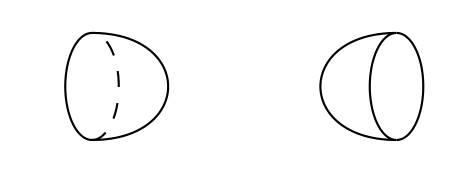
\includegraphics[width=0.2\textwidth]{img/birth-death.png}
\end{figure}
\end{example}

As an example of how cobordisms play in the wild, we have the following
lemma---which investigates the situation for \(0\)-manifolds.

\begin{lemma}[Cobordant zero and one dimensional manifolds]
\label{lem:cobordant-0-and-1-manifolds}
Two given compact \(0\)-manifolds without boundary are cobordant if and only if
they have the same number of points modulo \(2\). Moreover, any two compact
\(1\)-manifolds without boundary are cobordant.
\end{lemma}

\begin{proof}
Let's consider the case of a pair of \(0\)-manifolds \(\Sigma_0\) and
\(\Sigma_1\). Notice that since every pair of points can be connected by a
smooth curve, and every \(1\)-manifold with boundary has an even number of
boundary points\footnote{This is due to the fact that \(1\)-manifolds are
  \(C^{\infty}\)-isomorphic to a finite disjoint union of circles or intervals
  (see the appendix of~\cite{milnor}).}, it follows that
\(\Sigma_0\) and \(\Sigma_1\) are cobordant if and only if the disjoint union
\(\Sigma_0 \disj \Sigma_1\) has an even number of points.

For the second statement, one should recall that a compact \(1\)-manifold is the
disjoint union of circles. Then we can choose one of the manifolds to
attach copies of the death of a circle cobordism for each of its circles, and
attach birth of a circle cobordisms for each of its respective
circles of the other \(1\)-manifold. This construction yields a cobordism
between them.
\end{proof}

\subsection{Oriented Cobordisms}

Consider the following setup: let \(\Sigma\) be a closed submanifold of \(M\)
with codimension \(1\), where \(\dim M = n\). Assume both manifolds to be
oriented. Our goal will be to define the concept of orientation in a cobordism.

\begin{definition}[Positive normal]
\label{def:positive-normal-manifold}
Let \([v_1, \dots, v_{n-1}]\) be a positive basis for \(T_x \Sigma\) for any
given point \(x \in \Sigma\). We say that a tangent vector \(v \in T_x M\) is a
\emph{positive normal} if the induced basis \([v_1, \dots, v_{n-1}, v]\) for
\(T_x M\) is positive.
\end{definition}

Positive normals grant the possibility to distinguish boundaries of a manifold
by choosing something analogous to a time arrow.

\begin{definition}[In and out boundaries]
\label{def:in-out-boundaries}
If \(\Sigma\) is a connected component of \(\Bd M\), we call \(\Sigma\) an
\emph{in-boundary} if a positive normal points inwards relative to \(M\), and
otherwise an \emph{out-boundary}---when a positive normal points outward
relative to \(M\).
\end{definition}

The notion of an in and out boundary allows us to define the notion of an
oriented cobordism. From now on, \emph{a cobordism will always mean an oriented}
one, unless stated otherwise.

\begin{definition}[Oriented cobordism]
\label{def:oriented-cobordism}
Let \(\Sigma_{\text{in}}\) and \(\Sigma_{\text{out}}\) be compact
\((n-1)\)-manifolds without boundary. We define an \emph{oriented cobordism}
between them to be a triple \((M, \iota_{\text{in}}, \iota_{\text{out}})\),
where \(M\) is a smooth compact oriented \(n\)-manifold, and arrows
\[
\begin{tikzcd}
\Sigma_{\text{in}} \ar[r, "\iota_{\text{in}}"] &M
&\Sigma_{\text{out}} \ar[l, "\iota_{\text{out}}"']
\end{tikzcd}
\]
which are \(C^{\infty}\)-isomorphisms when restricted to the in and out boundary
of \(M\), respectively. We shall denote the oriented cobordism \(M\) as an
arrow \(M: \Sigma_{\text{in}} \nat \Sigma_{\text{out}}\).
\end{definition}

To give a better explanation to what was meant by the idea of choosing a time
arrow, notice that given a cobordism one can slice the resulting manifold with a
parametrization \(I \coloneq [0, 1]\), where at \(0\) one has a slice containing
the in-boundaries, while at \(1\) we have a slice forming the out-boundary. This
idea can come in handy for physical analogies.

\begin{example}[Cylinder cobordism]
\label{exp:cylinder-cobordism}
An important example of cobordism is that of a cylinder---it will play the role
of an identity morphism in the category of cobordisms that we have yet to
define. Let \(\Sigma\) be a compact oriented \((n-1)\)-manifold without
boundary. We define the \emph{cylinder cobordism} of \(\Sigma\) to be the triple
\((\Sigma \times I, \iota_{\text{in}}, \iota_{\text{out}})\), where we have
canonical inclusions
\[
\begin{tikzcd}
\Sigma \times 0
&\Sigma
\ar[l, "\iota_{\text{in}}"', "\iso", hook']
\ar[r, "\iota_{\text{out}}", "\iso"', hook]
&\Sigma \times 1
\end{tikzcd}
\]
that is, the cobordism from \(\Sigma\) to \(\Sigma\) itself.
\end{example}

In order to distinguish between two cobordisms, it is important to know when two
are equivalent or not. We address that as follows:

\begin{definition}[Equivalence of cobordisms]
\label{def:equivalence-of-cobordisms}
Given two cobordisms \(M, N: \Sigma_{\text{in}} \nat \Sigma_{\text{out}}\),
% \[
% \begin{tikzcd}
% \Sigma_{\text{in}} \ar[r, shift right=1.5, Rightarrow, "N"']
% \ar[r, shift left=1.5, Rightarrow, "M"]
% &\Sigma_{\text{out}}
% \end{tikzcd}
% \]
we say that \(M\) is \emph{equivalent} to the cobordism \(N\) if there exists an
orientation-preserving \(C^{\infty}\)-isomorphism \(\phi: M \isoto N\) such that
the following diagram commutes in \(\Man\):
\[
\begin{tikzcd}
&N &
\\
\Sigma_{\text{in}} \ar[ru] \ar[rd]
&
&\Sigma_{\text{out}} \ar[lu] \ar[ld]
\\
&M \ar[uu, "\phi", "\dis"']&
\end{tikzcd}
\]
\end{definition}

\section{Elements of Morse Theory}

An interesting tool for dealing with cobordisms is provided by Morse theory,
which we'll only scrap the surface and merely give some pertinent definitions
for our discussions.

\begin{definition}\label{def:non-degenerate-point-and-index}
Let \(f: M \to I\) be a \(C^{\infty}\)-morphism, and \(p \in M\) be a critical
point of \(f\). We call \(p\) a \emph{non-degenerate} point if there exists a
chart about \(p\) for which the local Hessian of \(f\) is
invertible. Furthermore, we define the \emph{index of \(f\) at \(p\)} to be the
number of \emph{negative eigenvalues} of the local Hessian.
\end{definition}

\begin{definition}[Morse maps]\label{def:morse-maps}
Let \(M\) be a smooth manifold. We say that a \(C^{\infty}\)-morphism
\(f: M \to I\) is a \emph{Morse map} if every critical point of \(f\) is
non-degenerate. If it happens to be the case that \(M\) is a manifold with
boundary, we shall further require that \(f^{-1}(\Bd I) = \Bd M\) and that the
boundary points \(\Bd I = \{0, 1\}\) are regular values of \(f\)---ensuring
that \(\Bd M\) has no critical points.
\end{definition}

The existence of Morse maps is ensured by the following theorem, which can be
found in~\cite{hirsch}:

\begin{theorem}\label{thm:morse-maps-are-dense}
For any manifold \(M\) and integer \(2 \leq r \leq \infty\), the collection of
Morse maps \(M \to I\) is dense in \(C^r(M, I)\).
\end{theorem}

\subsection{Decomposing \& Gluing Cobordisms}

We'll use the concept of gluing of spaces in order to provide the concept of
composition of cobordisms. For that, we have the following definition:

\begin{definition}[Gluing]\label{def:gluing-topological-spaces}
Let \(f: X \to Y\) and \(g: X \to Z\) be topological morphisms. We define the
\emph{gluing of \(Y\) and \(Z\) along \(X\)} to be the pushout
\[
\begin{tikzcd}
X \ar[d, "g"']
\ar[r, "f"]
\ar[rd, "\ulcorner", phantom, very near end]
&Y \ar[d] \\
Z \ar[r]
&Y \disj_X Z
\end{tikzcd}
\]
Explicitly, \(Y \disj_X Z\) is the quotient space of \(Y \disj Z\) where
\(y \sim z\) if and only if there exists a common \(x \in X\) such that
\(f x = y\) and \(g x = z\). For notational purposes, the gluing of \(Y\) and
\(Z\) along \(X\) can also be denoted by \(Y Z\) when \(X\) is implicitly
understood.
\end{definition}

Given a cobordism \(M: \Sigma_0 \nat \Sigma_1\), one can think how to slice
\(M\) so that we get a smooth submanifold \(\Sigma_t \subseteq M\) dividing
\(M\) into two. The first part should contain all in-boundaries of \(M\), while
the second should contain each out-boundary of \(M\). To that end, take a Morse
map \(f: M \to I\) such that \(f^{-1}(0) = \Sigma_0\) and
\(f^{-1}(1) = \Sigma_1\). We shall then define \(\Sigma_t\) as the preimage
\(f^{-1}(t) \subseteq M\), yielding two cobordisms
\[
M_{[0, t]} \coloneq f^{-1}([0, t]): \Sigma_0 \Longrightarrow \Sigma_t
\quad \text{ and } \quad
M_{[t, 1]} \coloneq f^{-1}([t, 1]): \Sigma_t \Longrightarrow \Sigma_1.
\]

The following theorem can be found in~\cite{hirsch} (page 153).

\begin{theorem}[Regular interval]\label{thm:regular-interval}
Let \(M: \Sigma_0 \nat \Sigma_1\) be a cobordism, and \(f: M \to I\) a Morse map
admitting no critical points and such that \(f^{-1}(0) = \Sigma_0\) and
\(f^{-1}(1) = \Sigma_1\). If \(\pi: \Sigma_0 \times I \epi I\) denotes the
canonical projection, then there exists a \(C^{\infty}\)-isomorphism
\(\phi: \Sigma_0 \times I \to M\) such that the following diagram commutes in
\(\Man\):
\[
\begin{tikzcd}
\Sigma_0 \times I \ar[r, "\phi", "\dis"'] \ar[rd, two heads, bend right, "\pi"']
&M \ar[d, "f"] \\
&I
\end{tikzcd}
\]
\end{theorem}

A relevant consequence of the regular interval theorem is the following:

\begin{lemma}\label{lem:regular-interval-decomposition-of-cobordism}
Let \(M: \Sigma_0 \nat \Sigma_1\) be a cobordism, and \(f: M \to I\) a Morse map
with \(f^{-1}(0) = \Sigma_0\) and \(f^{-1}(1) = \Sigma_1\). Then there exists
\(\varepsilon > 0\) and a \emph{decomposition}
\[
M = M_{[0, \varepsilon]} M_{[\varepsilon, 1]}
\]
such that \(M_{[0, \varepsilon]}\) is \(C^{\infty}\)-isomorphic to
\(\Sigma_0 \times I\). Analogously, there also exists a decomposition relating
to the out-boundary \(\Sigma_1\).
\end{lemma}

\begin{proof}
\(M\) being a manifold with boundary implies that \(f\) has no critical points
at the in and out boundaries of \(M\). Moreover, since \(f\) is a
\(C^{\infty}\)-morphism it follows that there must exist some pair
\(\varepsilon_1, \varepsilon_2 > 0\) for which \([0, \varepsilon_1]\) and
\([1 - \varepsilon_2, 1]\) are both sets of regular point of \(f\). We can then
conclude that both restrictions \(f|_{M_{[0, \varepsilon_1]}}\) and
\(f|_{M_{[1-\varepsilon_2, 1]}}\) are maps lacking critical points, and thus
satisfy the conditions to be Morse maps. Applying \cref{thm:regular-interval},
we obtain that \(M_{[0, \varepsilon_1]} \iso \Sigma_0 \times I\), and
\(M_{[1 - \varepsilon_2, 1]} \iso \Sigma_1 \times I\), and both claimed
decomposition of \(M\).
\end{proof}

\section{The Category \texorpdfstring{\(\Cob{n}\)}{n-cob}}

We would now like to construct a \emph{category of cobordisms} of a given
dimension \(n\). For that, our objects shall be compact oriented
\((n-1)\)-manifolds, but what about the arrows? A solution for this dilemma is
to use \emph{classes} of oriented cobordisms since we already know how to
distinguish one from the other.  In order for that to work, we shall define the
idea of \emph{composition} of cobordisms and show that if \(M = M_1 M_0\) is a
decomposition of a cobordism \(M\), then the composition of \(M_0\) and \(M_1\)
need to be \(M\)---that is, compositions and decompositions play nicely with
each other.

Our first step will be to define a gluing of any two cobordisms. For that, let
\(M_0: \Sigma_0 \nat \Sigma_1\) and \(M_1: \Sigma_1 \nat \Sigma_2\) be two
cobordisms, and consider Morse maps \(f_0: M_0 \to [0, 1]\) and
\(f_1: M_1 \to [1, 2]\). We'll try to relate the topological manifold
\(M_0 \disj_{\Sigma_1} M_1\)---which also comes with a continuous map
\(M_0 \disj_{\Sigma_1} M_1 \to [0, 2]\) induced by \(f_0\) and \(f_1\)---to a
cobordism of the form \(\Sigma_0 \nat \Sigma_2\). Choose \(\varepsilon > 0\)
such that the intervals \([1 - \varepsilon, 1]\) and \([1, 1 + \varepsilon]\)
are regular sets of \(f_0\) and \(f_1\), respectively. By
\cref{thm:regular-interval} we conclude that there are
\(C^{\infty}\)-isomorphisms
\(M_{[1 - \varepsilon, 1]} \iso \Sigma_1 \times [1 - \varepsilon, 1]\) and
\(M_{[1, 1 + \varepsilon]} \iso \Sigma_1 \times [1, 1 + \varepsilon]\), thus
there exists a \emph{topological} isomorphism
\[
M_{[1-\varepsilon, 1]} \disj_{\Sigma_1} M_{[1, 1 + \varepsilon]}
\iso \Sigma_1 \times [1 - \varepsilon, 1 + \varepsilon],
\]
whose restriction to \(M_{[1-\varepsilon, 1]}\) and \(M_{[1, 1 + \varepsilon]}\)
is a \(C^{\infty}\)-isomorphism. As a by-product one gets a smooth structure for
the whole gluing space \(M_0 \disj M_1\), which is itself a \emph{cobordism
  class}
\[
M_0 \disj M_1: \Sigma_0 \Longrightarrow \Sigma_2.
\]
We stress that such cobordism indeed represents a \emph{class} since the
\emph{choice} of the smooth structure \emph{isn't canonical}.

\begin{theorem}\label{thm:cobordism-classes-gluing}
Let \(M_0\) and \(M_1\) be cobordisms such that \(\Sigma\) is the out-boundary
of \(M_0\) and the in-boundary of \(M_1\). If \(\alpha\) and \(\beta\) are two
smooth structures for the gluing \(M_0 M_1\) along \(\Sigma\), there exists a
\(C^{\infty}\)-isomorphism \(\phi: (M_0 M_1, \alpha) \isoto (M_0 M_1, \beta)\)
such that \(\phi|_{\Sigma} = \Id_{\Sigma}\).
\end{theorem}

An important direct consequence of this theorem is that the gluing of cobordisms
has a unique smooth structure up to smooth isomorphism. Moreover, the smooth
structure should not depend on the choice of representative of the cobordism
class---and this is what we now show. To see this, consider any two cobordisms
\(M_0: \Sigma_0 \nat \Sigma_1\) and \(M_1: \Sigma_1 \nat \Sigma_2\), and suppose
there exists two cobordism equivalences \(\phi_0: M_0 \isoto M_0'\) and
\(\phi_1: M_1 \isoto M_1'\)---that is, we consider any other representatives
\(M_0'\) and \(M_1'\). Using the universal property of pushouts associated to
the gluings \(M_0 M_1\) and \(M_0' M_1'\), we get the following commutative
diagram in \(\Top\), where \(\phi\) is a unique \emph{topological} isomorphism:
\[
\begin{tikzcd}
\Sigma_1
\ar[d]
\ar[dd, bend right=40]
\ar[r]
\ar[rr, bend left=30]
&M_0
\ar[r, "\dis"'] \ar[d]
&M_0'
\ar[dd]
\\
M_1
\ar[r]
\ar[d, "\dis"]
&M_0 M_1
\ar[rd, dashed, "\phi", "\dis"']
&
\\
M_1' \ar[rr]
&
&M_0' M_1'
\end{tikzcd}
\]
The resulting map \(\phi\) restricts to a \(C^{\infty}\)-isomorphism between
manifolds on each of its factors. This shows that \(\phi\) is, in fact, an
equivalence of cobordisms:
\[
\begin{tikzcd}
&M_0' M_1' &
\\
\Sigma_0 \ar[ru] \ar[rd]
&
&\Sigma_2 \ar[lu] \ar[ld]
\\
&M_0 M_1 \ar[uu, dashed, "\phi", "\dis"'] &
\end{tikzcd}
\]
From now on we shall refer to cobordisms by their classes of equivalence.

With this we are finally ready to define precisely what we mean by the
composition of cobordisms classes:

\begin{definition}[Composition of cobordisms]\label{def:composition-cobordism}
Consider cobordisms classes \(M_0: \Sigma_0 \nat \Sigma_1\) and
\(M_1: \Sigma_1 \nat \Sigma_2\). We define the \emph{composition cobordism} of
\(M_0\) with \(M_1\) as the cobordism class \(M_0 M_1: \Sigma_0 \nat \Sigma_2\)
given by the gluing of \(M_0\) and \(M_1\) along \(\Sigma_1\).
\end{definition}

\begin{lemma}\label{lem:associativity-of-cobordism-composition}
The composition of cobordisms is associative.
\end{lemma}

\begin{proof}
Consider classes of cobordisms
\(\Sigma_0 \overset{M_0}\Longrightarrow \Sigma_1 \overset{M_1}\Longrightarrow
\Sigma_2 \overset{M_2} \Longrightarrow \Sigma_3\). To see that
\[
(M_0 M_1) M_2 = M_0 (M_1 M_2)
\]
it suffices to observe that: in \((M_0 M_1) M_2\) we first identify the common
boundary \(\Sigma_1\) of \(M_0\) and \(M_1\), and construct the smooth structure
around \(\Sigma_1\) as discussed before---further we identify \(\Sigma_2\) in
the same manner and obtain a gluing of \(M_0 \disj_{\Sigma_1} M_1\) with \(M_2\)
along \(\Sigma_2\). Notice that in this process we merely affected the smooth
structure around a small neighbourhood of \(\Sigma_1\) and \(\Sigma_2\), and
since those two boundaries are disjoint, this process can be done so that the
order in which we glue does not affect the resulting structure.
\end{proof}

Back to what we anticipated at \cref{exp:cylinder-cobordism}, we can now say in
what way the cylinder cobordisms act as an identity in the classes of
cobordisms:

\begin{lemma}
\label{lem:cylinder-cobordism-is-identity}
Given any cobordism \(M: \Sigma_0 \nat \Sigma_1\), if \(C_0\) and \(C_1\) denote
the cylinder cobordisms of \(\Sigma_0\) and \(\Sigma_1\) respectively, then
\[
C_0 M = M = M C_1.
\]
\end{lemma}

Now that we have objects and arrows that allow for composition, associativity,
and identities, we can finally define our desired category. For each
\(n \in \Z_{>0}\) we'll denote by \(\Cob{n}\) the category of \(n\)-dimensional
cobordisms, whose objects are compact oriented \((n-1)\)-manifolds without
boundary, and morphisms are classes of cobordisms between them.

\section{Monoidal Structure of \texorpdfstring{\(\Cob{n}\)}{n-cob}}

Notice that the coproduct given by the disjoint union in the category of
manifolds can be extended to a bifunctor
\(\disj: \Cob n \times \Cob n \to \Cob n\) by associating each pair of manifolds
\(\Sigma_0\) and \(\Sigma_1\) of \(\Cob n\) with the oriented \((n-1)\)-manifold
\(\Sigma_0 \disj \Sigma_1\) whose orientation is the canonical one---so that
inclusions are orientation preserving. Also, given two cobordisms
\(M: \Sigma_0 \nat \Sigma_1\) and \(N: \Theta_0 \nat \Theta_1\) we naturally
obtain a cobordism
\[
M \disj N: \Sigma_0 \disj \Theta \Longrightarrow \Sigma_1 \disj \Theta_1.
\]
Denoting by \(\emptyset_{n-1} \in \Cob n\) the empty \((n-1)\)-manifold, we know
that
\[
\emptyset_{n-1} \disj \Sigma \iso \Sigma \iso \Sigma \disj \emptyset_{n-1}
\]
for any \(\Sigma \in \Cob n\). Furthermore, if
\(\emptyset_n: \emptyset_{n-1} \nat \emptyset_{n-1}\) denotes the empty
\(n\)-cobordism, we also find that
\(M \disj \emptyset_n = M = \emptyset_n \disj M\) are the same cobordism
classes. This shows that \(\emptyset_{n-1}\) serves as a unit with respect to
the bifunctor \(\disj\) in the category \(n\)-cob. Thus we've obtained a
\emph{monoidal structure} \((\Cob n, \disj, \emptyset)\).

Back to the construction of cylinders, one can extend the ideas of
\cref{exp:cylinder-cobordism} to isomorphism between manifolds. Consider the
subcategory \(\cat C\) of \(\Man_{n-1}\), whose objects are compact oriented
\((n-1)\)-manifolds without boundary, and \(C^{\infty}\)-isomorphisms between
them. Let \(f: \Sigma_0 \isoto \Sigma_1\) be a morphism in \(\cat C\), and
define a cobordism \((\Sigma_0 \times I, i_0, f_1^{-1})\) where
\(i_0: \Sigma_0 \to \Sigma_0 \times I\) maps \(\Sigma_0\) to the in-boundary of
\(\Sigma_0 \times I\) while \(f_1^{-1}: \Sigma_1 \to \Sigma_0 \times I\) maps
\(\Sigma_1\) to the out-boundary of \(\Sigma_0 \times I\) via
\(x \mapsto (f^{-1} x, 1)\). Analogously, we define a cobordism
\((\Sigma_1 \times I, f, i_1)\). This construction is clear to make the diagram
\[
\begin{tikzcd}
&\Sigma_1 \times I &
\\
\Sigma_0 \ar[ru, "f"] \ar[rd, "i_0"']
& &\Sigma_1 \ar[lu, "i_1"'] \ar[ld, "f^{-1}"]
\\
&\Sigma_0 \times I  \ar[uu, "f \times \Id_I", "\dis"'] &
\end{tikzcd}
\]
commute, showing that \(f \times \Id_I\) is an isomorphism of cobordisms and
hence \(\Sigma_1 \times I \iso \Sigma_0 \times I\)---this cobordism class will
be denoted by \(\Cyl f\). This construction is functorial, which means that we
can define a functor \(\Cyl: \cat C \to \Cob n\) where we map the objects via
inclusions and \(f \mapsto \Cyl f\) as described above. Indeed, given another
arrow \(g: \Sigma_1 \isoto \Sigma_2\) of \(\cat C\), one has
\(\Cyl(g) \Cyl(f) = \Cyl(g f)\).

% \begin{proposition}
% \label{prop:iso-same-cobordism-class-iff-smooth-htpy}
% Parallel \(C^{\infty}\)-isomorphisms \(\Sigma_0 \para \Sigma_1\) induce
% equivalent cobordism classes \(\Sigma_0 \nat \Sigma_1\) if and only if they are
% smoothly homotopic.
% \end{proposition}

Since \(\disj\) is a coproduct in \(\Man\), there exists a natural isomorphism
\(\gamma: (- \disj -') \isonat (-' \disj -)\) in \(\Man_{n-1}\). This natural
transformation induces, via the cylinder construction, another natural
isomorphism
\[
T \coloneq \Cyl \circ \gamma: (- \disj -') \isonat (-' \disj -),
\]
this time in \(\Cob n\)---which we shall refer to as the \emph{twist
  cobordism}. The birth of \(T\) gives to \(\Cob n\) the structure of a
\emph{symmetric monoidal category} \((\Cob n, \disj, \emptyset, T)\).

\subsection{\texorpdfstring{\(\Cob 2\)}{2-cob}}

We shall be mostly interested in the case of two dimensional cobordisms, since
for \(n \geq 3\) the category \(\Cob n\) has a highly non-trivial
classification. We won't prove the classification theorem for \(\Cob 2\), which
can be found in both~\cite{kock,geiger} but nonetheless we at least state it
below. An important part of the proof is that any pair of \(2\)-dimensional
cobordisms are members of the same isomorphism class if and only if they have
the same number of connected components, that is, disjoint circles. This allows
us to see the skeleton of \(\Cob 2\) as \(\N\), where each number \(m \in \N\)
denotes an isomorphism class whose members have a total of \(m\) connected
components.

\begin{theorem}[Classification of \(\Cob 2\)]
\label{thm:classification-2-cob}
Every \(2\)-dimensional cobordism can be decomposed into the product of the
following set of generators:
\begin{figure}[h!]
\centering
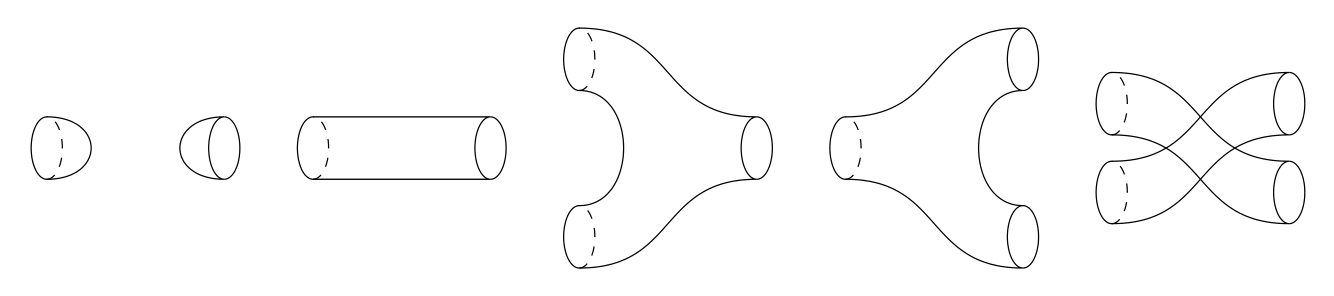
\includegraphics[width=0.8\textwidth]{img/2cob-generators.png}
\end{figure}

\noindent
Those generators are named, from left to right, the \emph{cup}, \emph{cap},
\emph{cylinder}, \emph{copants}, \emph{pants} and \emph{twist} cobordisms.
\end{theorem}

In the skeletal view of \(\Cob 2\), the cup is a map \(1 \nat 0\), the cap is
the map \(0 \nat 1\), the cylinder is \(1 \nat 1\), copants give \(2 \nat 1\),
pants correspond to \(1 \nat 2\), and the twist is a map \(2 \isonat 2\). An
extensive number of relations between these generators can be found in theorem
2.40 of~\cite{geiger}, which we ask the curious reader to take a look.

\section{Frobenius Algebras}

We now introduce the second main character of our study: Frobenius algebras.

\begin{definition}[Frobenius algebra]
\label{def:frobenius-algebras}
Let \((\cat M, \otimes, 1)\) be a monoidal category, and \(A \in \cat M\) be an
object. A tuple \((A, \mu, \eta, \delta, \varepsilon)\) is said to be a
\emph{Frobenius algebra} if it satisfies the following requirements:
\begin{itemize}\setlength\itemsep{0em}
\item The triple \((A, \mu, \eta)\) is a monoid, while
  \((A, \delta, \varepsilon)\) is a comonoid---where \(\mu\), \(\eta\),
  \(\delta\) and \(\varepsilon\) are arrows of \(\cat M\).

\item The diagram, encoding the so called \emph{Frobenius relation}, commutes in
  \(\cat M\):
\[
\begin{tikzcd}
(A \otimes A) \otimes A
\ar[dd, "\dis"']
&
&A \otimes A
\ar[ll, "\delta \otimes \Id_A"']
\ar[rr, "\Id_A \otimes \delta"]
\ar[d, "\mu"]
&
&A \otimes (A \otimes A)
\ar[dd, "\dis"]
\\
& &A \ar[d, "\delta"] & &
\\
A \otimes (A \otimes A)
\ar[rr, "\Id_A \otimes \mu"']
&
&A \otimes A
&
& (A \otimes A) \otimes A
\ar[ll, "\mu \otimes \Id_A"]
\end{tikzcd}
\]
\end{itemize}
\end{definition}

Pairings and copairings are structures that appear naturally in the context of
vector spaces. Here we'll generalise this concept to Frobenius algebras:

\begin{lemma}
\label{lem:(co)pairing-frobenius-algebra}
Let \((A, \mu, \eta, \delta, \varepsilon)\) be a Frobenius algebra in \((\cat M,
\otimes, 1)\). There exists morphisms \(\beta: A \otimes A \to 1\) and \(\theta:
1 \to A \otimes A\)---respectively called \emph{pairing} and
\emph{copairing}---such that the following two diagrams commute in \(\cat M\):
\[
\begin{tikzcd}
A \otimes A \otimes A
\ar[rr, "\mu \otimes \Id_A"]
\ar[d, "\Id_A \otimes \mu"']
& &A \otimes A \ar[d, "\beta"]
\\
A \otimes A \ar[rr, "\beta"']
& &1
\end{tikzcd}
\qquad
\qquad
\begin{tikzcd}
A \otimes A \otimes A
& &A \otimes A
\ar[ll, "\Id_A \otimes \delta"']
\\
A \otimes A \ar[u, "\delta \otimes \Id_A"]
& &1 \ar[ll, "\theta"] \ar[u, "\theta"']
\end{tikzcd}
\]
\end{lemma}

\begin{proof}
The pairing and copairing can be defined as \(\beta \coloneq \varepsilon \mu\)
and \(\theta \coloneq \delta \eta\). Indeed, these definitions allow for the
commutativity of the diagrams, since by \cref{def:(co)monoids} we have
\begin{gather*}
\beta (\Id_A \otimes \mu)
= (\varepsilon \mu) (\Id_A \otimes \mu)
= \varepsilon (\mu (\Id_A \otimes \mu))
= \varepsilon (\mu (\mu \otimes \Id_A))
= \beta (\mu \otimes \Id_A),
\\
(\delta \otimes \Id_A) \theta
= (\delta \otimes \Id_A) (\delta \eta)
= ((\delta \otimes \Id_A) \delta) \eta
= ((\Id_A \otimes \delta) \delta) \eta
= (\Id_A \otimes \delta) \theta.
\end{gather*}
\end{proof}

Our choice of pairing \(\beta\) and copairing \(\theta\) in the last proof is,
however, not unique. This motivates for the further restriction of a pairing to
that of a non-degenerate one: we say that \(\beta: A \otimes A \to 1\) is a
\emph{non-degenerate pairing} if and only if there exists
\(\theta: 1 \to A \otimes A\)---called a \emph{non-degenerate copairing}---such
that the diagram
\begin{equation}\label{eq:non-degenerate-pairing}
\begin{tikzcd}
A \otimes A \otimes A \ar[rr, "\beta \otimes \Id_A"]
& &1 \otimes A \iso A
\\
A \iso A \otimes 1 \ar[u, "\Id_A \otimes \theta"]
\ar[rru, bend right=20, "\Id_A"']
& &
\end{tikzcd}
\end{equation}
commutes in the ambient monoidal category \(\cat M\). As shown in~\cite{geiger}
lemma 3.21, given a non-degenerate pairing \(\beta\), its corresponding
non-degenerate copairing \(\theta\) is unique up to isomorphism. In fact, the
choice of \(\beta = \varepsilon \mu\) and \(\theta = \delta \eta\) satisfies
our non-degeneracy condition.

In our context we shall be mostly concerned with the case where the underlying
monoidal category of a Frobenius algebra is either \emph{braided} or
\emph{symmetric}. A crucial structure for our main theorem is that of
commutative Frobenius algebras, which we now define.

\begin{definition}[Commutative Frobenius algebra]
\label{def:commutative-frobenius-algebra}
We say that a Frobenius algebra \((A, \mu, \eta, \delta, \varepsilon)\) with an
underlying braided monoidal category \((\cat M, \otimes, 1, \gamma)\) is
\emph{commutative} if the following diagram commutes in \(\cat M\):
\[
\begin{tikzcd}
A \otimes A \ar[r, "\gamma"] \ar[rd, "\mu"'] &A \otimes A \ar[d, "\mu"] \\
&A
\end{tikzcd}
\]
Equivalently one could define \(A\) to be commutative if and only if \(\delta
\gamma = \delta\) (see lemma 3.27 of~\cite{geiger}).
\end{definition}

In order to define a category consisting of Frobenius algebras, we need first
consider how to construct morphisms between such objects. Given any two
Frobenius algebras \(A\) and \(A'\) in a symmetric monoidal category
\((\cat M, \otimes, 1, \gamma)\), we shall define a \emph{Frobenius algebra
  morphism} \(f: A \to A'\) to be a map that is both a monoid and comonoid
morphism.

With this definition at hand, we can define the category \(\Frob_{\cat M}\) of
Frobenius algebras of the symmetric monoidal category \(\cat M\). An important
full subcategory is that of commutative Frobenius algebras, which we'll denote
by \(\cFrob_{\cat M}\).

The particular case we'll be mostly interested in is that of Frobenius algebras
in the symmetric monoidal category \(\Vect_k\). As already noted early in the
text, in this ambient monoids are \(k\)-algebras, while comonoids are
\(k\)-coalgebras. Therefore, given a Frobenius algebra
\((A, \mu, \eta, \delta, \varepsilon)\) over \(\Vect_k\) there exists a
non-degenerate pairing \(\beta \coloneq \varepsilon \mu: A \otimes A \to k\) and
non-degenerate copairing \(\theta \coloneq \delta \eta: k \to A \otimes
A\). From lemma 2.1.13 of~\cite{kock} we conclude that \(A\) must be a finite
dimensional \(k\)-vector space. With this in hands we find that a Frobenius
algebra over \(\Vect_k\) is simply a finite dimensional \(k\)-algebra \(A\)
equipped with an associative\footnote{Given a \(k\)-algebra \(R\) and a pairing
  \(f: V \otimes W \to k\) where \(V\) is a right \(R\)-module and \(W\) is a
  left \(R\)-module, we say that \(f\) is \emph{associative} if for any pair
  \(x, y \in V\) and \(r \in R\) one has
  \(f(x \otimes (r \cdot y)) = f((x \cdot r) \otimes y)\).  } non-degenerate
pairing \(A \otimes A \to k\).

\section{Topological Quantum Field Theories}

The end our our brief journey is nigh, and we'll now get to know a fraction
of topological quantum field theory.

\begin{definition}
\label{def:tqft}
An \(n\)-dimensional \emph{topological quantum field theory} over a field \(k\)
is a symmetric monoidal functor \(Z: \Cob n \to \Vect_k\). The
collection of \(n\)-dimensional TQFT's over a field \(k\), and monoidal natural
transformations between them, forms a category
\[
\tqft{n}_k = \SymMon(\Cob n, \Vect_k).
\]
\end{definition}

The next theorem comes simultaneously as a great and bad news. Topological
quantum field theories can only realise finite dimensional spaces, which can be
great for computational purposes, but in general cannot withstand many important
physical applications that demand infinite dimensions.

\begin{theorem}
\label{thm:tqft-image-is-finite-dimensional}
Let \(Z \in \tqft{n}_k\) be any topological quantum field theory. Then
the image of \(Z\) is a \(k\)-vector space equipped with a
non-degenerate pairing---hence finite dimensional.
\end{theorem}

\begin{proof}
Let \(\Sigma \in \Cob n\) be any object, and denote by
\(\overline \Sigma \in \Cob n\) the manifold with opposite orientation. Consider
cobordisms \(M: \Sigma \disj \overline \Sigma \nat \emptyset_{n-1}\) and
\(N: \emptyset_{n-1} \nat \overline \Sigma \disj \Sigma\). Since \(Z\)
is a symmetric monoidal functor, these cobordisms induce \(k\)-linear morphisms
\(Z M: Z \Sigma \otimes Z \overline \Sigma \to k\)
and \(Z N: k \to Z \overline \Sigma \otimes Z
\Sigma\). Notice that we can decompose the cylinder \(\Sigma \times I\) as
\[
\Sigma \times I
\iso \big( (\Sigma \times I) \disj N \big) \big( M \disj (\Sigma \times I) \big),
\]
thus by applying \(Z\) we obtain the equality
\[
\Id_{Z \Sigma}
= \big( Z M \otimes \Id_{Z \Sigma} \big)
\big( \Id_{Z \Sigma} \otimes Z N \big)
\]
which is exactly the condition of commutativity imposed by
\cref{eq:non-degenerate-pairing}---thus \(Z M\) is a non-degenerate
pairing and \(Z N\) its respective non-degenerate copairing.
\end{proof}

We know from \cref{thm:classification-2-cob} that objects of \(\Cob 2\) are
disjoint unions of circles and can be uniquely assigned to natural numbers
\(n \in \N\) corresponding to \(\disj^n S^1\). Since a TQFT \(Z\) is a
monoidal functor, one has
\(Z(\disj^n S^1) = (Z S^1)^{\otimes n}\). From this we can
see that in order to understand how a \(2\)-dimensional topological quantum
field theory acts on a \(2\)-dimensional cobordism it is sufficient to
understand its action on a circle. To that end, we shall define more two
structures.

\begin{definition}[Free monoidal category over a Frobenius algebra]
\label{def:free-monoidal-cat-over-frobenius-algebra}
Let \((\chi, \otimes, 0)\) be a monoidal category with a skeleton generated by
\(1\)---that is, the objects of \(\chi\) are of the form
\(n = 1^{\otimes n}\)---and whose morphisms are generated by arrows
\(\mu: 2 \to 1\), \(\delta: 1 \to 2\), \(\eta: 0 \to 1\), and
\(\varepsilon: 1 \to 0\). Moreover, we impose that the following relations are
satisfied:
\begin{itemize}\setlength\itemsep{0em}
\item Commutativity: \(\mu (\Id \otimes \eta) = \Id = \mu (\eta \otimes \Id)\).

\item Cocommutativity:
  \((\Id \otimes \varepsilon) \delta = \Id = (\varepsilon \otimes \Id) \delta\).

\item Frobenius relations:
  \((\Id \otimes \mu) (\delta \otimes \Id) = \delta \mu = (\mu \otimes \Id) (\Id
  \otimes \delta)\).
\end{itemize}
That is, the tuple \((1, \mu, \eta, \delta, \varepsilon)\) is a Frobenius
algebra. With these conditions being satisfied, we shall call \(\chi\) a
\emph{free monoidal category over the Frobenius algebra} \(1\).
\end{definition}

As an immediate consequence of the imposed relations, we find that they also obey:
\begin{itemize}\setlength\itemsep{0em}
\item Associativity: \(\mu (\Id \otimes \mu) = \mu (\mu \otimes \Id)\).
\item Coassociativity: \((\delta \otimes \Id) \delta = (\Id \otimes \delta) \delta\).
\end{itemize}
This shows a strong relationship to the properties of the generator \(S^1\) and
\(\Cob 2\). We still however lack any kind of twist morphism. This will be
solved by the next definition.

\begin{definition}[Free symmetric monoidal category over a Frobenius algebra]
\label{def:free-symmetric-monoidal-cat-over-frobenius-algebra}
Let \((\chi, \otimes, 0)\) be a free monoidal category over a Frobenius algebra
\(1\). If we equip \(\chi\) with a braiding \(\gamma: 2 \isoto 2\) and impose
relations \(\mu \gamma = \mu\) and \(\gamma \delta = \delta\), it follows that
\((1, \mu, \eta, \delta, \varepsilon)\) is a commutative Frobenius algebra, and
we call \(\chi\) a \emph{free symmetric monoidal category over} \(1\).
\end{definition}

With this definition we have that \(\Cob 2\) is equivalent to any free symmetric
monoidal category over a Frobenius algebra, where the braiding \(\gamma\) plays
the role of the twist generator of \(\Cob 2\).

Since (symmetric) monoidal functors preserve the (symmetric) monoidal structure,
in particular, for any \(Z \in \tqft{2}_k\), the image
\(Z S^1\) of the commutative Frobenius algebra \(S^1 \in \Cob 2\) is
itself a commutative Frobenius algebra over the symmetric monoidal category
\(\Vect_k\).

\section{Equivalence Theorems}

At last we reached the climax, we shall now show the connections between what
we've been studying in the last few pages.

\begin{theorem}
\label{thm:monoidal-functor-categories-and-frobenius-algebras}
Let \(\chi\) be a free monoidal category over a Frobenius algebra \(1\). If
\((\cat M, \otimes, e)\) is any monoidal category, then there exists a natural
isomorphism
\[
\Mon(\chi, \cat M) \iso \Frob_{\cat M}.
\]
\end{theorem}

\begin{proof}
Let \(G: \chi \to \cat M\) be any monoidal functor, and define the Frobenius
algebra \(G(1) = F\). From the definition of \(G\) we know that any object
\(n \in \chi\) has an image \(G n = F^{\otimes n}\). For the arrow generators,
we find their image under \(G\) satisfy all the needed conditions for the tuple
\((F, G \mu, G \eta, G \delta, G \varepsilon)\) to be a Frobenius algebra.

On the other hand, if we start with the Frobenius algebra
\(F \in \Frob_{\cat M}\), we can associate to it the monoidal functor
\(\chi \to \cat M\) that maps \(1\) to \(F\) and the arrow generators
corresponding to the important arrows of \(F\) as described in the last
paragraph. With this we arrive exactly at the functor \(G\).

Let \(N, N' \in \Mon(\chi, \cat M)\) be any two monoidal functors, and consider a
monoidal natural transformation \(\tau: N \nat N'\) between them. Denote by
\(F\) and \(F'\) the Frobenius algebras \(N(1)\) and \(N'(1)\), respectively. For
any object \(n \in \chi\), the morphism \(\tau_n\) is merely the \(n\)-th tensor
product of the map \(\tau_1: F \to F'\). From naturality of \(\tau\), the
generators of \(\chi\) induce the following commutative diagrams:
\[
\begin{tikzcd}
{F \otimes F} \ar[r, "\tau_2"] \ar[d, "N \mu"']
&{F' \otimes F'} \ar[d, "N' \mu"]
\\
{F} \ar[r, "\tau_1"']
&{F'}
\end{tikzcd}
%
\qquad
%
\begin{tikzcd}
F \ar[r, "\tau_1"]
&F'
\\
e \ar[u, "N \eta"] \ar[r, equal, "\tau_0"']
&e \ar[u, "N' \eta"']
\end{tikzcd}
%
\qquad
%
\begin{tikzcd}
F \ar[r, "\tau_1"] \ar[d, "N \delta"']
&F' \ar[d, "N' \delta"]
\\
F \otimes F \ar[r, "\tau_2"']
&F' \otimes F'
\end{tikzcd}
%
\qquad
%
\begin{tikzcd}
e \ar[r, equal, "\tau_0"]
&e
\\
F \ar[u, "N \varepsilon"] \ar[r, "\tau_1"']
&F' \ar[u, "N' \varepsilon"']
\end{tikzcd}
\]
The first two commutative squares say that \(\tau_1\) is a monoid morphism,
while the last two squares say that \(\tau_1\) is a comonoid morphism. By
definition we conclude that \(\tau_1\) is a morphism of Frobenius algebras.

At last, if we start with a given morphism of Frobenius algebras, we must use
the data provided by its action on the generating arrows and the above
commutative squares to construct a monoidal natural transformation. With these
steps we find again the same transformation \(\tau\), as wanted.
\end{proof}

We now include an additional requirement of symmetry to the monoidal
category and extend the proof of
\cref{thm:monoidal-functor-categories-and-frobenius-algebras} to our needs.

\begin{theorem}
\label{thm:sym-monoidal-functor-categories-and-frobenius-algebras}
Let \(\chi\) be a free symmetric monoidal category over a commutative Frobenius
algebra \(1\) with braiding \(\gamma\). If \((\cat M, \otimes, e, \sigma)\) is
any symmetric monoidal category, then there exists a natural isomorphism
\[
\SymMon(\chi, \cat M) \iso \cFrob_{\cat M}.
\]
\end{theorem}

\begin{proof}
From previous considerations, for any symmetric monoidal functor
\(\tau: \chi \to \cat M\) we have \(\tau \gamma = \sigma\) and we obtain a
commutative Frobenius algebra
\((\tau(1), \tau \mu, \tau \eta, \tau \delta, \tau \varepsilon)\).

From the proof of \cref{thm:monoidal-functor-categories-and-frobenius-algebras},
any commutative Frobenius algebra in \(\cat M\) can be used to define a unique
monoidal functor \(\chi \to \cat M\). Moreover, the braiding \(\gamma\) induces
a symmetric structure to such fuctor. Therefore the chosen commutative Frobenius
algebra uniquely defines a unique object in \(\SymMon(\chi, \cat M)\).

For arrows, given any monoidal natural transformation \(\tau: S \nat S'\)
between symmetric monoidal functors \(S, S' \in \SymMon(\chi, \cat M)\). Denote
\(F \coloneq S(1)\) and \(F' \coloneq S'(1)\). By the last theorem we obtain a
morphism of Frobenius algebras \(\tau_1: F \to F'\) which trivially satisfies the
commutativity of the square
\begin{equation}\label{eq:twists-commutativity-sym-mon-func}
\begin{tikzcd}
F \otimes F
\ar[d, "S \gamma = \sigma"']
\ar[r, "\tau_2"]
&F' \otimes F' \ar[d, "S' \gamma = \sigma"] \\
F \otimes F \ar[r, "\tau_2"']
&F' \otimes F'
\end{tikzcd}
\end{equation}
This shows that \(\tau_1\) is in fact a morphism between commutative Frobenius
algebras. Now if we start with a morphism in \(\cFrob_{\cat M}\) we can---as
described in the last proof---obtain a unique monoidal functor
\(\chi \to \cat M\). This monoidal functor will however be symmetric, due to the
data provided by the additional commutative square
\cref{eq:twists-commutativity-sym-mon-func}. With this we prove the wanted
natural equivalence of categories.
\end{proof}

Now our main result comes merely as a free corollary of the last theorem.

\begin{corollary}
\label{cor:equivalence-2tqft-commutative-frobenius}
There exists a natural isomorphism
\[
\tqft{2}_k \iso \cFrob_{\Vect_k}.
\]
\end{corollary}

\begin{proof}
Notice that since \(\tqft{2}_k = \SymMon(\Cob 2, \Vect_k)\) we can apply
\cref{thm:sym-monoidal-functor-categories-and-frobenius-algebras} and obtain the
wanted natural isomorphism.
\end{proof}

With this we reach the end of our hasty expedition through the deep forest of
topological quantum field theory, of which we only ventured its borders. I'm
grateful for the reader who spent the time to read until the very end. For those
who got motivated to read further, a possible continuation would
be~\cite{lurie-tqft}---which I didn't use as a reference, but wish I could.

\printbibliography
\end{document}

%%% Local Variables:
%%% mode: latex
%%% TeX-master: t
%%% End:
